\documentclass{article}
\usepackage{amsmath}
\usepackage{amssymb}
\usepackage{enumitem}
\usepackage{algorithm}
\usepackage{listings}
\usepackage{color,xcolor}
\usepackage[T1]{fontenc}
\usepackage{etoolbox}
\usepackage{multicol}
\usepackage{geometry}
\usepackage[colorlinks=true,linkcolor=blue,urlcolor=red,bookmarksopen=true]{hyperref}
\usepackage{tikz, pgfplots, tkz-euclide,calc}
    \usetikzlibrary{patterns,snakes,shapes.arrows,3d,patterns.meta,angles,quotes}
    \geometry{
        total = {160mm, 237mm},
        left = 25mm,
        right = 35mm,
        top = 30mm,
        bottom = 30mm,
      }

\usepackage{tcolorbox}
     \tcbuselibrary{listings,skins}

\newcommand{\enter}{\raisebox{-1.8pt}{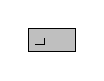
\begin{tikzpicture}[scale=0.3]
    \draw[thin,fill=lightgray] (0,0) rectangle (2,1);
    \draw (0.3,0.3) -- (0.7,0.3)--(0.7,0.6);     
\end{tikzpicture}}}

\definecolor{HIMAmuda}{HTML}{01D1FD}
\definecolor{HIMAtua}{HTML}{02016A}
\definecolor{HIMAabu}{HTML}{CBCBCC}
\definecolor{pgray}{rgb}{0.5,0.5,0.5}
\definecolor{pblue}{rgb}{0.13,0.13,1}
\definecolor{pgreen}{rgb}{0,0.5,0}
\definecolor{pred}{rgb}{0.9,0,0}
\definecolor{pgrey}{rgb}{0.46,0.45,0.48}
\definecolor{pcyan}{HTML}{D4EFFC}
\definecolor{lblue}{HTML}{00AEEF}
\definecolor{input}{HTML}{AAE1FA}
\definecolor{bg}{rgb}{0.95, 0.95, 0.92}
\definecolor{vscode}{HTML}{282A36}
\definecolor{PastelGreen}{HTML}{77DD77}

\newcommand{\inputscan}[1]{\raisebox{0pt}[1pt]{\colorbox{darkgray}{#1}}}

\usepackage{listings}

\lstdefinestyle{Liang}{
language=Java,
showspaces=false,
showtabs=false,
breaklines=true,
showstringspaces=false,
breakatwhitespace=true,
commentstyle=\color{pgray},
keywordstyle=\color{pblue},
stringstyle=\color{pgreen},
basicstyle=\small\ttfamily,
frame=single,
backgroundcolor=\color{pcyan},
escapeinside={(*}{*)},}

\lstdefinestyle{output}{
    language=Java,
    backgroundcolor=\color{vscode},
    basicstyle=\small\ttfamily\color{white},
    frame=none,
    escapeinside={(*}{*)},
    showspaces=false,
    showtabs=false,
    breaklines=true,
    showstringspaces=false,
    breakatwhitespace=true,
    keywordstyle=\color{white},
    }

\lstdefinestyle{standard}{
    language=Java,
    showspaces=false,
    showtabs=false,
    breaklines=true,
    showstringspaces=false,
    breakatwhitespace=true,
    commentstyle=\color{pgray},
    keywordstyle=\color{pblue},
    stringstyle=\color{pgreen},
    basicstyle=\small\ttfamily,
    frame=single,
    backgroundcolor=\color{bg},
    escapeinside={(*}{*)},}
\lstset{style=Liang}

\newtcblisting{RunCode}[1][enhanced,drop shadow]{
    arc=0pt, outer arc=0pt,
    boxsep=1pt,
    boxrule=2pt,
    auto outer arc,
    colback=vscode,
    colframe=bg,
    listing only, 
    listing style=output,
    title=\color{black}Ex. Output,
    #1
    }
\newtcblisting{RunCode+}[1][enhanced,drop shadow]{
    arc=0pt, outer arc=0pt,
    boxsep=1pt,
    boxrule=2pt,
    auto outer arc,
    colback=vscode,
    colframe=bg,
    listing only, 
    listing style=output,
    #1
    }

\newtcolorbox{hint}[1][]{
    colback=PastelGreen!5!white, 
    colframe=PastelGreen!75!black,
    fonttitle=\bfseries, 
    colbacktitle=PastelGreen!85!black,
    enhanced, 
    attach boxed title to top left={yshift=-2mm}, 
    title=Hint,
    #1
}

\newtcolorbox{req}[1][]{
    colback=lblue!5!white, 
    colframe=lblue!75!black,
    fonttitle=\bfseries, 
    colbacktitle=lblue!85!black,
    enhanced, 
    attach boxed title to top left={yshift=-2mm}, 
    title=Input,
    #1
}

\newtcolorbox{out}[1][]{
    colback=HIMAtua!5!white, 
    colframe=HIMAtua!75!black,
    fonttitle=\bfseries, 
    colbacktitle=HIMAtua!85!black,
    enhanced, 
    attach boxed title to top left={yshift=-2mm}, 
    title=Output,
    before upper=\renewcommand\thempfootnote{\Roman{mpfootnote}},
    #1
}

\renewcommand{\thesubsection}{\arabic{subsection}}
\newcommand{\R}{\mathbb{R}}
\newcommand{\Z}{\mathbb{Z}}

\title{\textbf{Week 4 Assigment}}
\date{30 September 2024}
\author{Teosofi H.A \& Hafidz M.}

\begin{document}
    \maketitle
    \pagenumbering{gobble}

    \section*{Tugas Mandiri}
    \begin{enumerate}[label=\textbf{\arabic*.}]
        \item \textbf{(Kalkulus)}\\
        Diberikan fungsi sepotong-sepotong berikut:
        \[f(x)=\begin{cases}
            \displaystyle \frac{\sin x}{x} &,\,0\leq x\leq\pi\\
            \\
            x+1 &,\,-2<x< 0\\ 
            \\
            \displaystyle\frac{x^3+6x^2+11x+6}{x+2} &,\,-4\leq x\leq-2
        \end{cases}\]
        Perbaiki fungsi bilangan real tersebut agar menjadi fungsi yang kontinu di seluruh domainnya. Kemudian buatlah program yang menerima input berupa nilai $x$ dan mengeluarkan nilai $f(x)$.
        \begin{req}
            \begin{itemize}
                \item $x:=$ variabel input dari sebuah fungsi.\\
                $x\in\mathcal{D}(f)$
            \end{itemize}
        \end{req}
        \begin{out}
            \begin{itemize}
                \item $f(x):=$ nilai dari fungsi $f$ untuk nilai $x$.\\
                $y\in\mathcal{R}(f)$
            \end{itemize}
        \end{out}
        \begin{RunCode}
x = (*\inputscan{-2} \enter*)
f(-2) = -1
        \end{RunCode}
        \begin{RunCode+}
x = (*\inputscan{4} \enter*)
Nilai x tidak di dalam domain fungsi.      
        \end{RunCode+}
        \begin{RunCode+}
x = (*\inputscan{0} \enter*)
f(0) = 1  
        \end{RunCode+}
        \newpage
        \item \textbf{(Logika Matematika)}\\
        Bacalah puisi berikut:
        \begin{quote}
            ``\textit{Andaikan pikiran dan hati sejalan\\
            Alangkah indah dunia dalam pandangan\\
            Dirimu yang dulu buatku nyaman\\
            Namun ternyata itu hanyalah khayalan}''
            \begin{quote}
                ``\textit{Hatiku terasa lesu dan pilu\\
                Tak ada yang salah dari hal itu\\
                Yang salah hanyalah diriku\\
                Yang pernah denganmu bertemu}''
            \end{quote}
            ``\textit{Jika saja aku tak pernah tahu\\
            Mungkin hatiku tak kan membeku\\
            Namun kini ku telah memilih berjumpa\\
            Kujalani segalanya meski terasa hampa}''
        \end{quote}
        Buatlah program sekreatif mungkin yang menerima input berupa sebuah pilihan "bertemu" atau "tidak bertemu" dan mengeluarkan output berupa simpulan dari puisi tersebut.
        \begin{req}
            \begin{itemize}
                \item $p:=$ pilihan input "benar" atau "salah".\\
                $p\in\{0,1\}$
            \end{itemize}
        \end{req}
        \begin{out}
            Menampilkan kalimat simpulan dari pilihan yang telah dipilih.
        \end{out}
    \end{enumerate}
\end{document}